\documentclass{report}
\title{\Large  Physics 20 - Lissajous figures and beats}
\author{\large Shubh Agrawal, \normalsize\emph{Class of 2022}}
\date{\small October 10, 2018}
\usepackage[a4paper,top=2cm, left=2.5cm,width=13cm,bottom=2cm,right=2.5cm]{geometry}
\usepackage{amsthm, amsmath, amssymb, tipa, graphicx, caption, subcaption, float}

\begin{document}

\maketitle
\subsection*{Introduction}
To analyze Lissajous figures, a problem-specific simulation was implemented in Python. Functions of directed modules \texttt{numpy} and \texttt{matplotlib} were used to generate supplementary graphs, which ease comprehension. Several variations of the model were run to hypothesize answers to the provided questions. The source code is available as an attachment (\emph{Assignment1.py}). 

\subsection*{Question of closed Lissajous figures for rational frequency ratios}
We investigate the hypothesis that the $X$ vs $Y$ curves are closed figures when the ratio of frequencies, i.e. $f_X/f_Y$, is a rational number. For the first set of simulations, the amplitudes $A_X$ and $A_Y$ are taken to be the same and equal to 10 units; the phase difference $\phi$ is taken to be zero. The interval gap $\Delta t$ and number of simulations $N$ are noted with the frequencies in caption.
\begin{figure}[H]
	\centering
	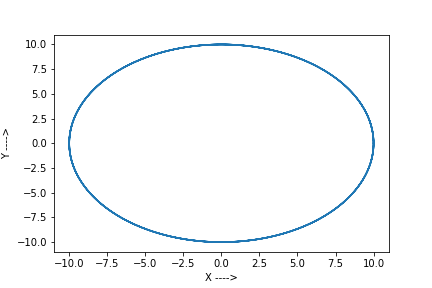
\includegraphics[width = \textwidth]{20-20.png}
	\label{closed1}
	\caption{$f_X=20$, $f_Y=20$, $N=20000$, $\Delta t=0.00001$}
\end{figure}
\begin{figure}[H]
	\centering
	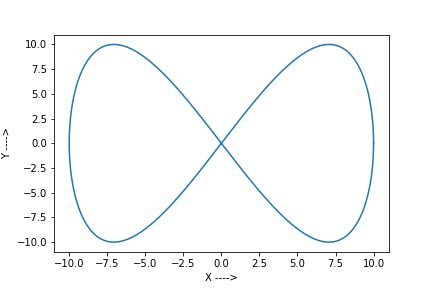
\includegraphics[width = \textwidth]{10-20.png}
	\label{closed2}
	\caption{$f_X=10$, $f_Y=20$, $N=10000$, $\Delta t=0.00001$}
\end{figure}
\begin{figure}[H]
	\centering
	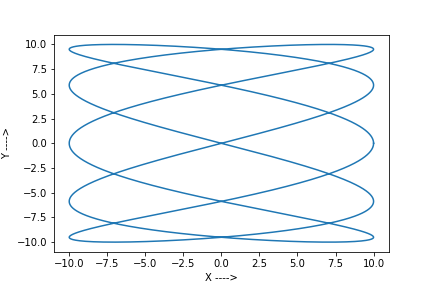
\includegraphics[width = \textwidth]{50-20.png}
	\label{closed3}
	\caption{$f_X=50$, $f_Y=20$, $N=10000$, $\Delta t=0.00001$}
\end{figure}
\begin{figure}[H]
	\centering
	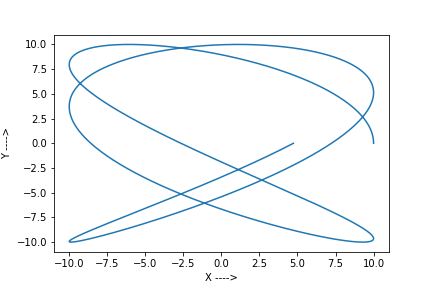
\includegraphics[width = \textwidth]{sqrt2.png}
	\label{open1}
	\caption{$f_X=\sqrt{2}$, $f_Y=1$, $N=20000$, $\Delta t=0.0001$}
\end{figure}
\begin{figure}[H]
	\centering
	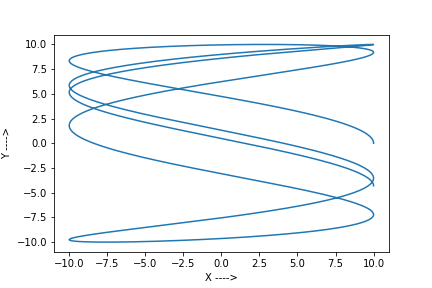
\includegraphics[width = \textwidth]{pi.png}
	\label{open2}
	\caption{$f_X=10$, $f_Y=\pi$, $N=5000$, $\Delta t=0.0001$}
\end{figure}
\pagebreak

For this set of simulations, phase difference is also varied as noted in the captions. The unit is radians.
\begin{figure}[H]
	\centering
	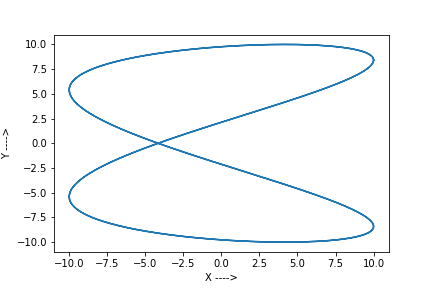
\includegraphics[width = \textwidth]{phase2010.png}
	\label{phase1}
	\caption{$f_X=20$, $f_Y=10$, $N=2000$, $\Delta t=0.0001$, $\phi=1$}
\end{figure}
\begin{figure}[H]
\centering
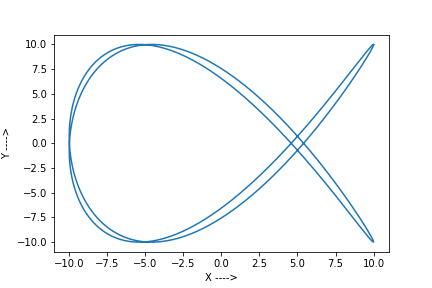
\includegraphics[width = \textwidth]{phase1015.png}
\label{phase2}
\caption{$f_X=10$, $f_Y=15$, $N=2000$, $\Delta t=0.0001$, $\phi=1.5$}
\end{figure}
\pagebreak

For our final set of simulations, the amplitudes $A_x$ and $A_y$ are varied as noted in caption.

\begin{figure}[H]
	\centering
	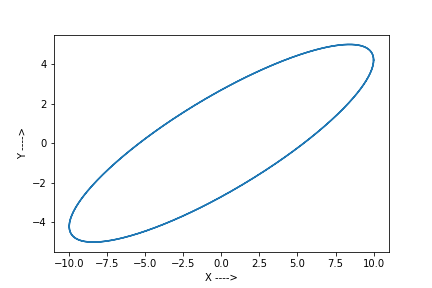
\includegraphics[width = \textwidth]{amp105.png}
	\label{amp1}
	\caption{$f_X=20=f_Y$, $A_X=10$, $A_Y=5$, $N=1000$, $\Delta t=0.0001$, $\phi=1$}
\end{figure}

\begin{figure}[H]
	\centering
	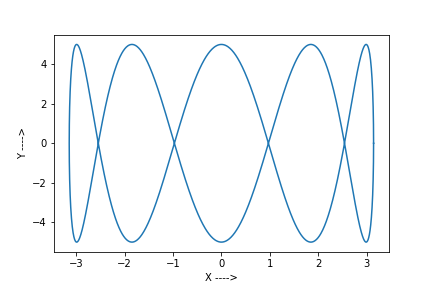
\includegraphics[width = \textwidth]{amp_pi.png}
	\label{phase1}
	\caption{$f_X=5$, $f_Y=25$, $A_X=\pi$, $A_Y=5$, $N=2000$, $\Delta t=0.0001$, $\phi=0$}
\end{figure}
It is notable that, irrespective of the values of and relations between other variables, we consistently get a well defined closed curved for rational values of $f_X/f_Y$. Our conclusion is also promoted by the two counter examples.

\subsection*{Dependency of $X$-$Y$ curves on frequency ratio}
The methodology used includes the analysis of the graph nature under different $f_X/f_Y$, after it (the ratio) is reduced to the lowest terms. For the set of curves, other factors are not varied to amplify only the result of ratio variation. The amplitudes $A_X$, $A_Y$ in these simulations are constant and equal to 10; the phase difference is 0.5 radians.
\begin{figure}[H]
	\centering
	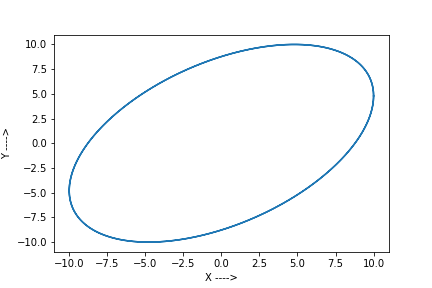
\includegraphics[width = \textwidth]{ratio1.png}
	\label{ratio1}
	\caption{$f_X=10$, $f_Y=10$, $f_X/f_Y=1=1/1$, $N=20000$, $\Delta t=0.00001$.  Only one single elliptical curve (one lobe) is modeled}
	\end{figure}
\begin{figure}[H]
	\centering
	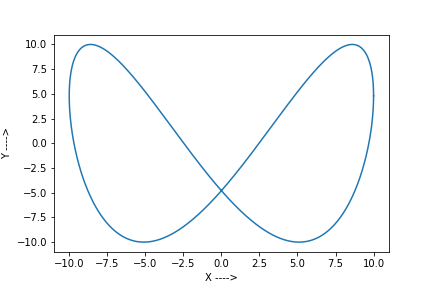
\includegraphics[width = \textwidth]{ratio2.png}
	\label{ratio2}
	\caption{$f_X=10$, $f_Y=20$, $f_X/f_Y=1/2$, $N=10000$, $\Delta t=0.00001$. Two horizontal lobes, along +X direction. No vertical divisions.}
\end{figure}
\begin{figure}[H]
	\centering
	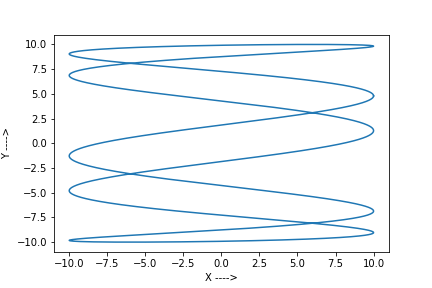
\includegraphics[width = \textwidth]{ratio3.png}
	\label{ratio3}
	\caption{$f_X=50$, $f_Y=10$, $f_X/f_Y=5/1$, $N=10000$, $\Delta t=0.00001$. Five vertical lobes along Y direction observed. Horizontal direction does not have such distinctions (one ``lobe'').}
\end{figure}
\begin{figure}[H]
	\centering
	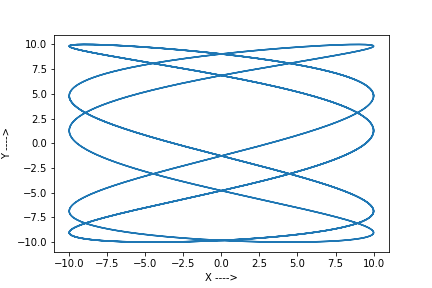
\includegraphics[width = \textwidth]{ratio4.png}
	\label{ratio4}
	\caption{$f_X=250$, $f_Y=100$, $f_X/f_Y=5/2$, $N=5000$, $\Delta t=0.00001$. 5 vertical lobe divisions and 2 horizontal lobe divisions produced.}
\end{figure}
\begin{figure}[H]
	\centering
	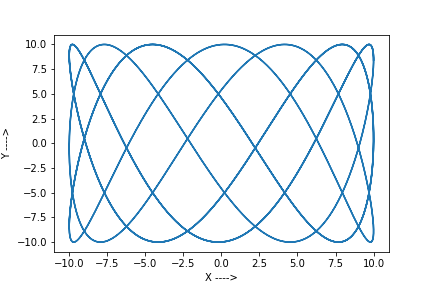
\includegraphics[width = \textwidth]{ratio5.png}
	\label{ratio5}
	\caption{$f_X=15$, $f_Y=35$, $f_X/f_Y=3/7$, $N=5000$, $\Delta t=0.00001$, $\phi=1$ (for clearer view). 3 vertical lobes and 7 horizontal lobes formed.}
\end{figure}
We already know that the curves are closed for rational ratios and else open. It is further noted that, after having reduced the rational ratio $f_X/f_Y$ to the lowest form $S/T$ ($s$ and $t$ are co-prime integers), the number of vertical lobes are $S$, and $T$ is the number of horizontal nodes. Alternatively, we can say that there are $S-1$ nodes along the Y axis direction, and $T-1$ nodes along the X direction.

\subsection*{Dependency of $X$-$Y$ curves on phase difference $\phi$}
As implied by the question, the methodology for this dependency analysis would include keeping factors, other than $\phi$, constant to increase readability. So, we take $f_X=f_Y=10$ and $A_X=A_Y=5$ (units). As computation involves the trigonometric functions $\sin$ and $\cos$, it is indicated that the nature of $\phi$ can be periodic and intimately related to the value of the constant $\pi$. 

For the first set of simulations, the aim was to determine if the shape of the X Y closed-figure curve is periodic on $\phi$, and, if yes, what could be the period. Models were made for gradual increase; it was noted that the graph is the same for all $n\pi + \phi$, where $n$ is an integer. The hypothesis was also verified by running a graduated loop cycle, and some of its outputs are presented below.

\begin{figure}[H]
	\centering
	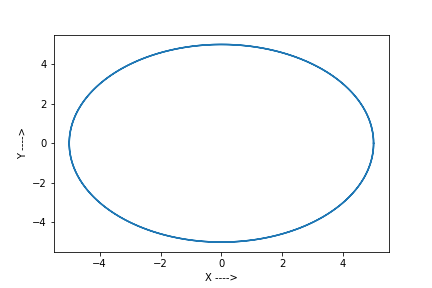
\includegraphics[width = \textwidth]{phi1.png}
	\label{phi1}
	\caption{$\phi=0$, $N=20000$, $\Delta t=0.00001$. Note that the ellipse axes are along the cardinal directions.}
\end{figure}

\begin{figure}[H]
\centering
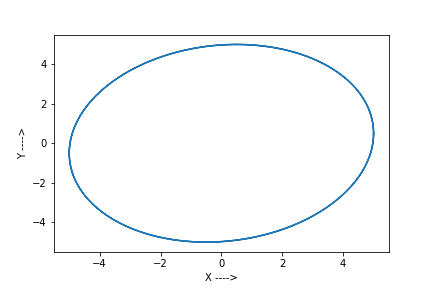
\includegraphics[width = \textwidth]{phi2.png}
\label{phi2}
\caption{$\phi=0.1$, $N=20000$, $\Delta t=0.00001$. As we increase the phase difference (still below $\pi/2$) we note that the axes start rotating counter clockwise, as the $\phi$ is used in $Y$ expression.}
\end{figure}

\begin{figure}[H]
	\centering
	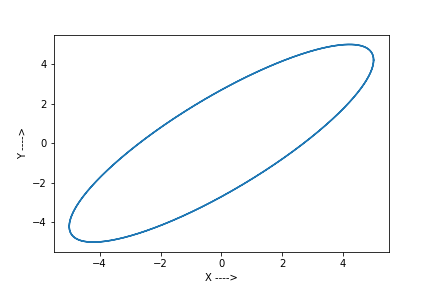
\includegraphics[width = \textwidth]{phi3.png}
	\label{phi3}
	\caption{$\phi=1<\pi/2<\pi$, $N=20000$, $\Delta t=0.00001$. See previous caption.}
\end{figure}


\begin{figure}[H]
	\centering
	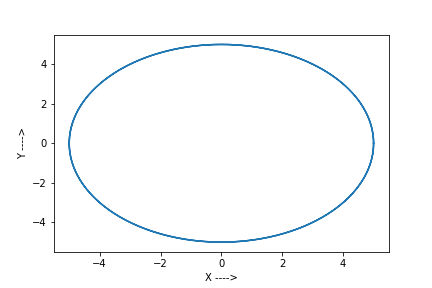
\includegraphics[width = \textwidth]{phi4.png}
	\label{phi4}
	\caption{$\phi=\pi$, $N=20000$, $\Delta t=0.00001$. This is similar to the graph for zero phase difference, indicating that the period of nature can be $\pi$.}
\end{figure}


\begin{figure}[H]
	\centering
	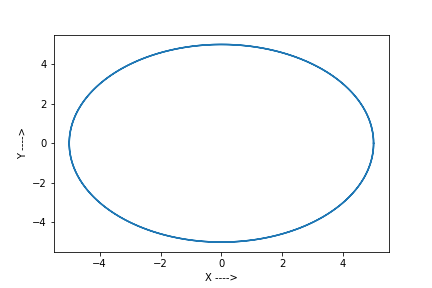
\includegraphics[width = \textwidth]{phi5.png}
	\label{phi5}
	\caption{$\phi=-2\pi$, $N=20000$, $\Delta t=0.00001$. Example of negative integer multiple.}
\end{figure}

\begin{figure}[H]
	\centering
	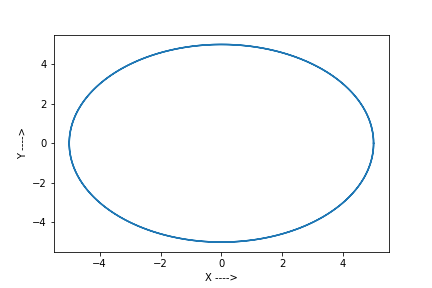
\includegraphics[width = \textwidth]{phi6.png}
	\label{phi6}
	\caption{$\phi=5648\pi$, $N=20000$, $\Delta t=0.00001$. Example of arbitrary integer multiple.}
\end{figure}

Thus, the period must be $\pi$. For further analysis, the fact that the axis rotate counter-clockwise is used. A gradual increase is taken within the bounds of 0 and $n\pi$ (one period), keeping in mind the possible inflection points such as the multiples of $\pi$, especially the ones across which the derivative nature of the trigonometric functions varies.


\begin{figure}[H]
	\centering
	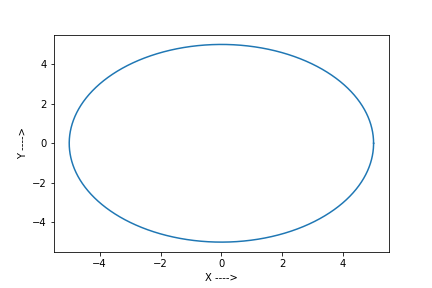
\includegraphics[width = \textwidth]{phiA.png}
	\label{phiA}
	\caption{$\phi=0$, $N=10000$, $\Delta t=0.00001$. No angle, axes are along cardinal directions.}
\end{figure}

\begin{figure}[H]
	\centering
	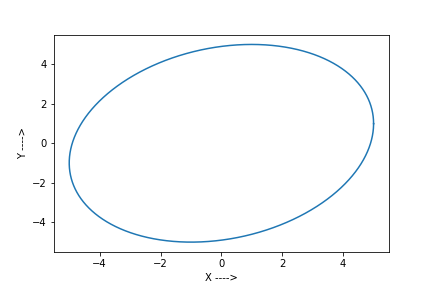
\includegraphics[width = \textwidth]{phiB.png}
	\label{phiB}
	\caption{$\phi=0.2<\pi/4$, $N=10000$, $\Delta t=0.00001$. Slight anticlockwise rotation of ellipse axes.}
\end{figure}

\begin{figure}[H]
	\centering
	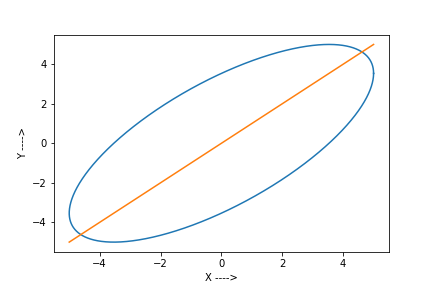
\includegraphics[width = \textwidth]{phiC.png}
	\label{phiC}
	\caption{$\phi=\pi/4$, $N=10000$, $\Delta t=0.00001$. We note that the axes of the ellipse are now $x=y$ and $x=-y$. $x=y$ is plotted for reference; it might seem that the line is offset, which is a result of using different scales for both axes.}
\end{figure}

\begin{figure}[H]
	\centering
	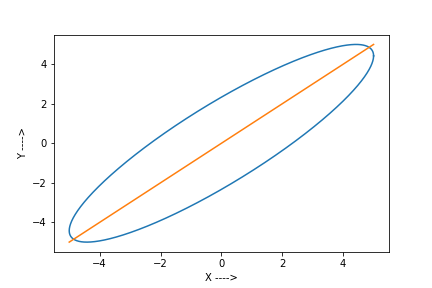
\includegraphics[width = \textwidth]{phiD.png}
	\label{phiD}
	\caption{$\phi=\pi/4<\pi/4+0.3<\pi/2$, $N=10000$, $\Delta t=0.00001$. As  $\phi$ is further increased, the major axis is still in the same orientation but the length of the minor axis starts to decrease. This appears as the ellipse shrinking or contracting.}
\end{figure}

\begin{figure}[H]
	\centering
	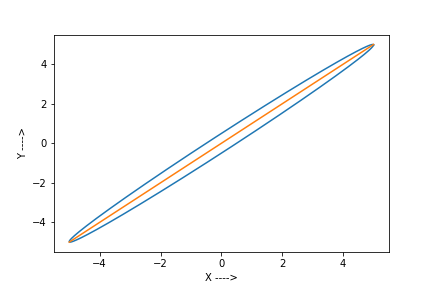
\includegraphics[width = \textwidth]{phiE.png}
	\label{phiE}
	\caption{$\phi=\pi/4<\pi/2-0.1<\pi/2$, $N=10000$, $\Delta t=0.00001$. Further example of previous situation.}
\end{figure}\

\begin{figure}[H]
	\centering
	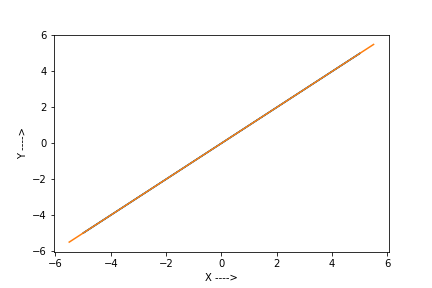
\includegraphics[width = \textwidth]{phiF.png}
	\label{phiF}
	\caption{$\phi=\pi/2$, $N=10000$, $\Delta t=0.00001$. The length of minor axis becomes zero, such that the ellipse coincides withe the axis.}
\end{figure}

\begin{figure}[H]
	\centering
	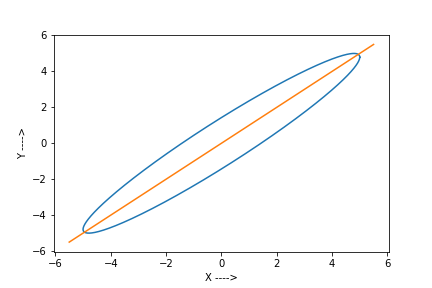
\includegraphics[width = \textwidth]{phiG.png}
	\label{phiG}
	\caption{$\phi=\pi/2+0.29<3\pi/4$, $N=10000$, $\Delta t=0.00001$. On increasing $\phi$, the figure again starts to ``expand'', as the minor axis length increases (it actually expands in the opposite direction, but as the figure is symmetric it is perceived to the same).}
\end{figure}
\begin{figure}[H]
	\centering
	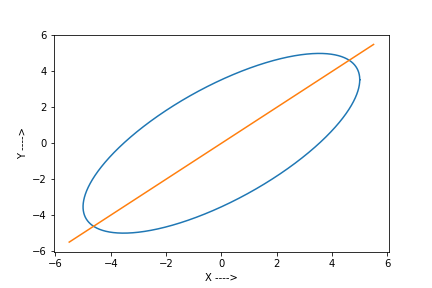
\includegraphics[width = \textwidth]{phiH.png}
	\label{phiH}
	\caption{$\phi=3\pi/4$, $N=10000$, $\Delta t=0.00001$. At $3\pi/4$, we find the same figire as $\pi/2$, consistent with the period $\pi$.}
\end{figure}

\begin{figure}[H]
	\centering
	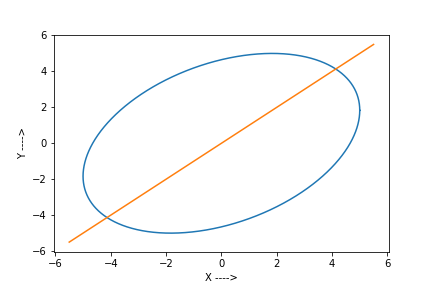
\includegraphics[width = \textwidth]{phiI.png}
	\label{phiI}
	\caption{$\phi=3\pi/4+0.41$, $N=10000$, $\Delta t=0.00001$. As we go beyond $3\pi/4$, the figure starts to rotate clockwise back to its original state, consistent with its periodic nature.}
\end{figure}

\begin{figure}[H]
	\centering
	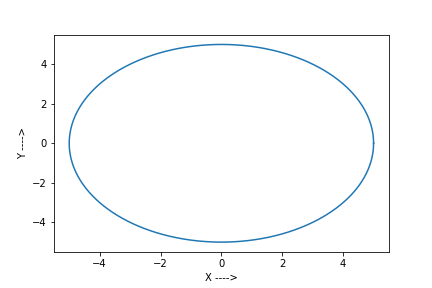
\includegraphics[width = \textwidth]{phiJ.png}
	\label{phiJ}
	\caption{$\phi=\pi$, $N=10000$, $\Delta t=0.00001$. We get the same initial state.}
\end{figure}

Now, it is conclude that Lissajous figures / $X-Y$ curves have a period of $\pi$. Additionally, it is note that within a period, from the lower bound to the upper bound, the figure first rotates counterclockwise such that its major axis goes from $y=0$ (X axis) at $\phi=0$ to $y=x$ at $\phi=\pi/4$. Beyond that, the minor axis starts shrinking resulting in a straight line segment figure at $\phi=\pi/2$. Then, the process of changes in nature happen in reverse from $\pi/2$ till $\pi$, i.e., the ellipse expands, then the major axis rotates back to $y=0$ (at $\pi$) from $y=x$.
\subsection*{Phenomenon of Beats}
To demonstrate beats, unequal values of $f_X$ and $f_Y$ were used. Similar to previous collections, models for a variety of amplitude/phase values are presented. The values of the carrier frequency $(\omega_1+\omega_2)/2$ and the modulation frequency $(\omega_1-\omega_2)$ (or modulus of) are also specified in caption.

The question of why the modulation frequency is $(\omega_1-\omega_2)$, and not $(\omega_1-\omega_2)/2$ as expected mathematical is as follows. First, consider the proposition that a \emph{negative} value of amplitude does not physically imply a different system than its positive counterpart, i.e., $A_w \equiv -A_w$ physically. This statement is true as amplitude is just the maximum distance of the particle (undergoing oscillatory motion) from its mean position, and the sign of distance just depends on our coordinate frame of reference.\\ 
Now, for the first half-cycle (starting from 0 with positive slope) of the $\sin$ (or $\cos$, depending on initial phase) of $(\omega_1-\omega_2)/2$, the  algebraic values of effective amplitude is non-negative, i.e., $A_{\text{eff}}\geq 0$. For the second half-cycle, the algebraic values of effective amplitude is non-positive. However, it is equivalent to the first half-cycle, as the sine curve is symmetric about all zero-points (like the origin). Thus, the frequency effectively doubles (analogous to use of modulus function), and it becomes $2*(\omega_1-\omega_2)/2=(\omega_1-\omega_2)$.
\begin{figure}[H]
	\centering
	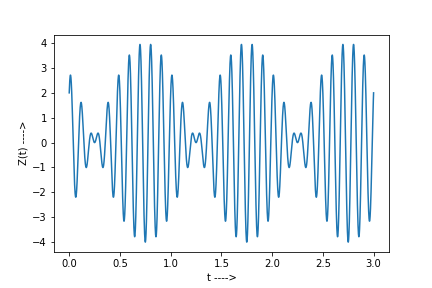
\includegraphics[width = \textwidth]{beats1.png}
	\label{beats1}
	\caption{$f_X=10$, $f_Y=9$, $A_X=A_Y=2$, $N=10000$, $\Delta t=0.0003$, $\phi=0$, $(\omega_1+\omega_2)/2=19\pi$, $(\omega_1-\omega_2)=2\pi$}
\end{figure}  
\begin{figure}[H]
	\centering
	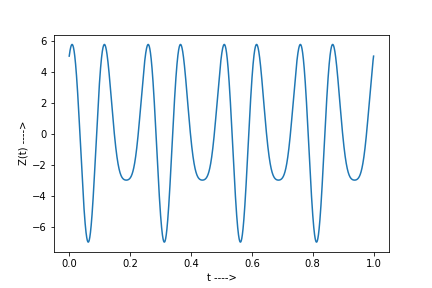
\includegraphics[width = \textwidth]{beats2.png}
	\label{beats2}
	\caption{$f_X=8$, $f_Y=12$, $A_X=5$ $A_Y=2$, $N=10000$, $\Delta t=0.0001$, $\phi=0$, $(\omega_1+\omega_2)/2=20\pi$, $(\omega_1-\omega_2)=8\pi$}
\end{figure}  
\begin{figure}[H]
	\centering
	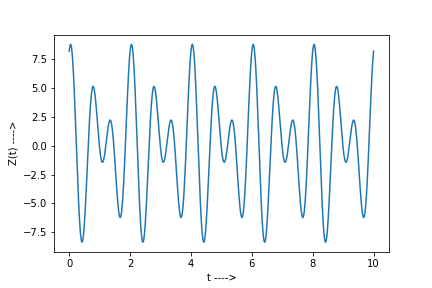
\includegraphics[width = \textwidth]{beats3.png}
	\label{beats3}
	\caption{$f_X=1$, $f_Y=1.5$, $A_X=4$, $A_Y=5$, $N=10000$, $\Delta t=0.001$, $\phi=1$, $(\omega_1+\omega_2)/2=2.5\pi$, $(\omega_1-\omega_2)=\pi$}
\end{figure}  
\subsection*{Experience of Python}
As Rossum notes, Python is highly readable due to whitespace indentation and easier representation of frequently used commands/functions. Being used to programming in Java which is complied, I noticed that Python debugging/implementing is significantly quicker. Polymorphic variables are a boon; when correctly used, they provide excellent flexibility.

Extensibility is a key component which makes Python powerful. The predefined packages like \texttt{numpy} and \texttt{matplotlib} are widely applicative. Additional aid is the re-usability provided by the object-oriented approach: similar processes can be overloaded, and the same code is run for various simulations.
\end{document}